%! TEX root = 'main.tex'
\section{Finding Kernel TOCTOU Bugs}
\label{sec:ktoctou-experiment}


This section presents our fuzzing tool \toolname for kernel-level TOCTOU vulnerability and the results we obtained on Windows, especially from the Win32k graphical subsystem.

Kernel-level TOCTOU vulnerabilities are subtle. It is not intuitive for the developers to be aware of those double fetches. They are not apparent errors such as buffer overflow that the compiler-based method~\cite{nagarakatte2015everything}~\cite{zhang2010intpatch} can detect. It is even harder to spot than the use-after-free vulnerability that code emulation or run-time checks can expose~\cite{feist2016finding}~\cite{chen2020savior}~\cite{lee2015preventing}~\cite{serebryany2012addresssanitizer}. As described in \autoref{sec:ktoctou-background}, the exploit needs to win the race with the kernel in high speed, and only by chance that it can trigger the vulnerability. From previous research works and vulnerabilities' publicly available information, the cause of kernel-level TOCTOU vulnerability is either due to historical reasons that a kernel module is highly coupled with user libraries or because of sloppy coding style. 

However, this vulnerability has a solid memory access pattern, namely, two reads from kernel to userspace. It is not convenient to observe such a pattern either from user programs or the kernel. The most intuitive way is to use a virtual machine. Previous work such as~\cite{jurczyk2013identifying}~\cite{bochspwnreloaded} utilize a full software emulated virtual machine Bochs~\cite{lawton2003bochs}, which parses and executes each instruction without hardware virtualization assistant or dynamic binary translation.  It is straight forward to instrument the operating system kernel, and it discovers many double-fetch vulnerabilities~\cite{jurczyk2013identifying}~\cite{bochspwnreloaded}. However, due to the nature of full software emulation, the virtual machine runs extremely slow. So it is not easy to make a comprehensive test, especially with GUI programs, because GUI needs a prompt response.

As previously described in \autoref{sec:ktoctou-background}, the SMAP feature is an ideal way of monitoring kernel-to-user-memory behavior. The goal is to check if the same address is being read twice by one system call.

However, the difficulty lies in recovering the system from a fatal SMAP exception.  Because of its original intention, the operating system should crash when it receives such an exception. We tried different methods to cancel a SMAP exception, such as disabling it at CR4.SMAP or temporarily disable it through setting EFLAGS.AC. None of them works.  Fortunately, setting the faulting page to kernel-mode is one way to satisfy the processor so far. Subsequently, we want to release the page back to user-mode as soon as possible not to lose track of the kernel.



\textbf{\textit{Single Step Trap.}} It is the soonest way to get back control. Through setting the trap flag (TF) in the EFLAGS register, the processor stops at every instruction. After setting the faulting page to kernel-mode to recover from the SMAP exception, we want the processor to stop at the next instruction. So we can release the protected page and continue the kernel.

 For the single-step trap, the processor automatically sets the resume flag (RF) in the EFLAGS register so that the handler itself will not be interrupted on every instruction. Because we use a hypervisor, the single-step trap triggers a VM exit. In the event handler, we try to clear the TF or set the RF in the guest EFLAGS and then resume the virtual machine. However, the RF flag does not work properly under such circumstances; the single-step still comes in.

 \textbf{\textit{Breakpoint}} We decide to take an alternative approach that writes a software breakpoint directly on the next instruction. We first parse the current instruction's length and then write a byte 0xcc to it. Next, we record the information of this access and let the kernel continue. When the hypervisor gets the debug trap, we fix it with the original byte, release the protected page, and then resume the virtual machine to re-execute the faulting instruction.



\textbf{\textit{Results.}} We found a few double fetch candidates; ~\autoref{table:doubleread} in~\autoref{sec:ktoctou-evaluation} gives a glimpse of the problem. This method has advantages over the binary static analysis. In the x86 instruction set, there are a few addressing modes of accessing memory, such as \textit{absolute}, \textit{register}, \textit{register + offset}, which makes it difficult to identify the same address from the syntax perspective.  For example, in~\autoref{fig:doublefetch}, it needs to trace both ECX and EDX registers and, in some cases, need to get user input to calculate the final address eventually. In \toolname, each user address visited is reported through the hardware mechanism SMAP. Therefore, it can accurately locate every double fetch within a system call.


\begin{figure}[th]
  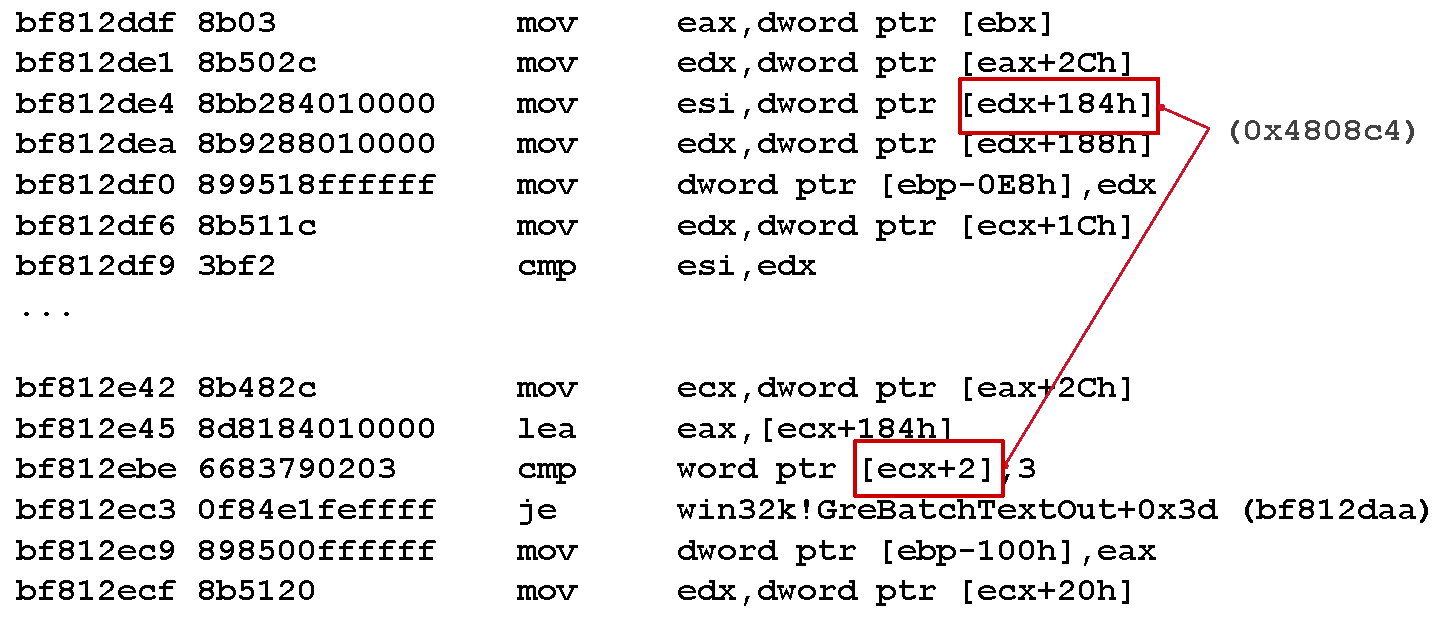
\includegraphics[width=0.47\textwidth]{figures/doublefetch}
  \centering
  \caption{CR3 0x6d40320; TEB 0x7ffdd000; EIP 0xbf812de4 and 0xbf812e4b read the same user-mode address 0x4808c4 within one system call.}
  \label{fig:doublefetch}
\end{figure}


Whether those bugs can further become vulnerabilities is need to analyze case by case. However, a significant potential of those accesses is not within a try-catch block. It may lead to a local denial-of-service (DOS) attack if the attacker frees the user page right ahead of the access.
